\documentclass[paper=a4,fontsize=11pt]{report}	% For KOMA, use scrartcl


% ------------------------------------------------------------------------------
% Imports and Packages
% ------------------------------------------------------------------------------
\usepackage[a4paper,includeheadfoot,margin=1in]{geometry}

\usepackage[english]{babel}
\usepackage[protrusion=true,expansion=true]{microtype}	
\usepackage{amsmath,amsfonts,amsthm,amssymb} % Math
\usepackage{float} % For [H] centering
\usepackage{graphicx} % For images
\usepackage[style=ieee, sorting=none, backend=biber]{biblatex} % Citation

\usepackage{setspace}
\doublespacing


% Table formatting
\usepackage{booktabs}
\usepackage[table,xcdraw]{xcolor}
\usepackage{longtable}

\addbibresource{references.bib}

% ------------------------------------------------------------------------------
% Definitions (do not change this)
% ------------------------------------------------------------------------------

\newcommand{\HRule}[1]{\rule{\linewidth}{#1}} 	% Horizontal rule

\graphicspath{{../images/}}

\makeatletter							% Title
\def\printtitle{%						
    {\centering \@title\par}}
\makeatother									

\makeatletter							% Author
\def\printauthor{%					
    {\centering \large \@author}}				
\makeatother							


% ------------------------------------------------------------------------------
% LaTeX Variables and Shortcuts
% ------------------------------------------------------------------------------

\newcommand{\me}{Sahil Manojkumar Pattni}
\newcommand{\setA}{\{A\}}
\newcommand{\setB}{\{B\}}
\newcommand{\abrule}{\setA\rightarrow\setB}


% ------------------------------------------------------------------------------
% Metadata (Change this)
% ------------------------------------------------------------------------------

\title{	\normalsize \textsc{Final Year Dissertation} 	% Subtitle
		 	\\[2.0cm]								% 2cm spacing
			\HRule{0.5pt} \\						% Upper rule
			\LARGE \textbf{{Market Basket Analysis with Graph Theory}}	% Title
			\HRule{2pt} \\ [0.5cm]		% Lower rule + 0.5cm spacing
			\normalsize \today			% Todays date
		}



\author{
		Sahil M. Pattni\\	
		Bachelor of Science with Honours in Computer Science\\
        Supervised by Dr. Neamat El Gayar \\
}


\begin{document}
% ------------------------------------------------------------------------------
% Maketitle
% ------------------------------------------------------------------------------
\thispagestyle{empty}		% Remove page numbering on this page

\begin{figure}[H]
\centering

\includegraphics[scale=0.22]{hw_logo.png}
\end{figure}

\printtitle					% Print the title data as defined above
  	\vfill


\printauthor				% Print the author data as defined above





% ------------------------------------------------------------------------------
% Begin document
% ------------------------------------------------------------------------------
\thispagestyle{empty}		% Remove page numbering on this page
\pagebreak
\hspace{0pt}
\vfill
\section*{Declaration}
I, \me, confirm that this work submitted for assessment is my own and is expressed in my own words. Any uses made within it of the works of other authors in any form (e.g., ideas, equations, figures, text, tables, programs) are properly acknowledged at any point of their use. A list of the references employed is included.
\\\\Date: \today
\\Signed: \me

\vfill
\hspace{0pt}
\pagebreak

\newpage\section*{Abstract}
In this digital age, data is being generated and collected at an unprecedented rate, with data analytics employed by corporations and small businesses alike to produce actionable insights, reduce costs, optimize operations and increase revenue. Association rules allow us to identify relationships between products that can provide insights into customer spending habits and product perception.


In this study, a minimum spanning tree (MST) will be generated from a transactional database such that only the strongest relationships between products remain. A clustering algorithm will be applied to this MST to identify high co-purchase segments, and association rules will then be extracted from these segments. \textbf{TODO: ADD MORE}

% Table of Contents
\newpage\tableofcontents\newpage





\setcounter{page}{1}		% Set page numbering to begin on this page
\chapter{Introduction}
\section{Motivation}
For businesses such as groceries, hypermarkets, and retail outlets that deal with the trade of heterogeneous physical assets, operations such as inventory management and product placement play an instrumental role in determining the business' financial success. These involve asking questions such as:
\begin{itemize}
\item Which products should be placed at the entrance of the store? Which should be placed closer to the exit?
\item Which products will benefit the most by being placed at eye-level?
\item Which products should be placed next to each other to maximize the purchase volume?
\end{itemize}
One way to find optimal solutions to such queries is to employ the use of Association Rule Mining (also known as Market Basket Analysis). This set of techniques assess frequent itemsets (e.g. from sales data) and generate association rules between products. 
A prime example of the utility of association rules is the urban legend of \textit{"Beers and Pampers"}, where a company allegedly studied their point-of-sale data and found a strong association between the purchase of diapers and a particular brand of beer during a certain time. With \textit{diapers} as the antecedent and \textit{beer} as the consequent, this rule can be written as:
\[
\{\textit{Diapers}\} \rightarrow \{\textit{Beer}\}
\]
This is an example of a single-element rule, where both the antecedent and consequent are sets that contain only one element each. Several algorithms exist for association rule mining, most prominently the Apriori Algorithm \cite{apriori} and FP-Growth \cite{fp_growth}, however these algorithms tend to generate an overwhelming amount of rules, rendering it inconvenient for the end-user to extract actionable information from the ruleset. This paper proposes to improve upon an existing method (see: Section \ref{sec:mst paper})  that derives association rules from minimum spanning trees.

\section{Aims}
The aim of this paper is to improve upon the aforementioned method by introducing a method that allows for the generation of multi-element association rules (i.e. rules where either/both the antecedent and consequent of the rule contain more than one element).

\section{Objectives}
The research objectives for this paper are as described below:
\begin{enumerate}
\item Acquire a suitable dataset upon which the study can be conducted.
\item Construct an affinity graph from the chosen dataset.
\item Explore and evaluate MST extraction algorithms.
\item Identify and evaluate methodologies for generating multi-element association rules from an MST.
\item Extract MST from the graph and generate association-rules using the chosen methodologies.
\item Evaluate the generated association rules against the rules generated by the Apriori Algorithm.
\end{enumerate}

\section{Structure (?)}
Maybe describe the structure of the document here?





\chapter{Background}



\section{Graph Theory}
\begin{figure}[H]
\centering
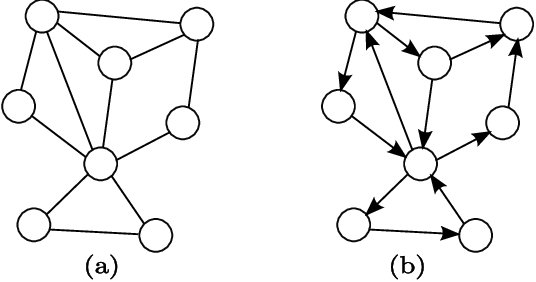
\includegraphics[scale=1.5]{graph-example}
\caption{Undirected and Directed Graphs}
\label{fig:graph.example}
\end{figure}
In discrete mathematics and more specifically - graph theory, a graph is a data structure that contains a set of nodes (i.e. vertices) connected by lines (i.e. edges).  These edges may be directed - such as in Figure \ref{fig:graph.example}:(a), or undirected - such as in Figure \ref{fig:graph.example}:(b). A graph $G$ with a set of vertices $V$ and a set of edges $E$ can be represented via the notation $G = (V,E)$. For the scope of this project,  we will be building undirected graphs, where the weight between two vertices is the same in both directions.
\subsection{Minimum Spanning Trees}
Given an undirected $G = (V,E)$,  a \textit{spanning tree} can be described as a subgraph that is a tree which includes all the vertices $V$ of $G$ with the minimum number of edges required. A \textit{minimum spanning tree} (MST) is the spanning tree with the smallest sum of edge weights.  This means that if the graph has $n$ vertices, each spanning tree - including the minimum spanning tree - will have $n-1$ edges. There are two widely used algorithms to extract the minimum spanning tree from a graph: Prim's algorithm and Kruskal's algorithm.
\subsection{Prim's Algorithm}
Independently discovered by three authors,  Prim's algorithm \cite{prims}\cite{prims_og}\cite{prims3} is a greedy algorithm\footnote{Selecting the locally optimal choice at each iteration of the solution} to find the minimum spanning three of an undirected,  weighted graph $G$. To successfully implement the algorithm, three sets need to maintained: a set of \textit{discovered} edges, and two sets of vertices: a set of \textit{undiscovered} vertices, and a set of \textit{discovered} vertices.  Figure \ref{fig:prim} illustrates Prim's algorithm being applied to a graph. The algorithm is as follows:\\
Initialize an empty set of discovered edges: $E$, and two sets of vertices: an empty set $D$ of the discovered vertices, and $UD$ as the set of undiscovered vertices.
\begin{itemize}
\item Pick an arbitrary vertex as a starting point (in the case of Figure \ref{fig:prim}, the top right node). Add this vertex to $D$ and remove it from $UD$.
\item While $UD$ is not empty:
	\begin{itemize}
	\item Find the edge $e_i$ with the smallest weight such that it connects together a vertex $V_1$ in $D$ and $V_2$ in $UD$ (to avoid forming cycles).
	\item Append $V_2$ to $D$ and remove it from $UD$ (i.e. $V_2$ is now discovered).
	\item Append $e_i$ to $E$.
	\end{itemize}
\end{itemize}
Once $D$ contains all the vertices of $G$, the algorithm terminates, and the set $D$ represents the minimum spanning tree, and $\sum\limits_{i=1}^n e_i$ is the weight of the MST. The time complexity of this algorithm is $O(V^2)$.
\begin{figure}[H]
\centering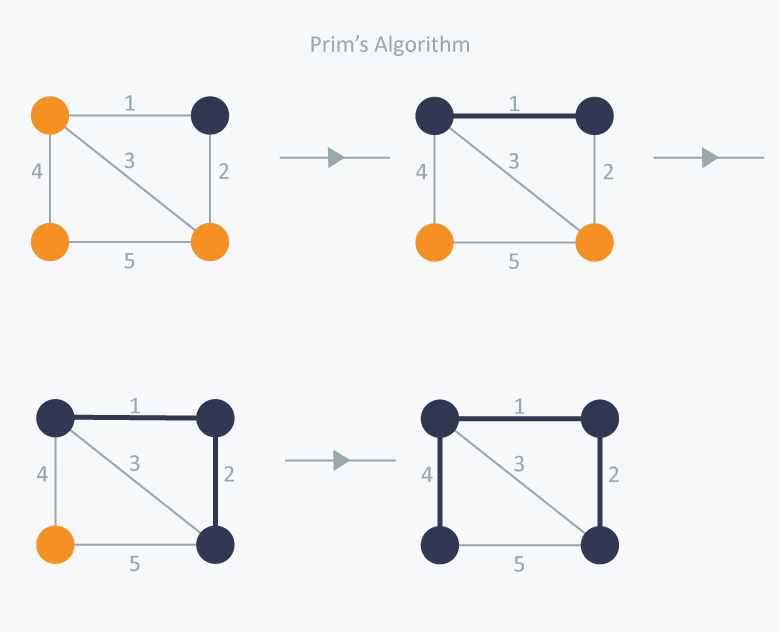
\includegraphics[scale=0.5]{prims}
\caption{Prim's Algorithm applied to a graph \cite{prim-pic} }\label{fig:prim}
\end{figure}

\subsection{Kruskal's Algorithm}
Another greedy algorithm,  Kruskal's algorithm \cite{kruskal} also extracts the MST from a graph.  Unlike Prim's algorithm, Kruskal's doesn't select an edge that connects directly to the already built spanning tree, but rather picks the global optimal solution. The algorithm is as follows:\\
Maintaining a set of edges $E$, and an initially empty set of chosen edges $C$:
\begin{itemize}
\item Sort the set of edges $E$ in ascending order.
\item While the number of elements in $C$ is not $n-1$:
	\begin{itemize}
	\item Select the smallest edge $e_i$ from $E$.
	\item If adding it does not form a cycle with the spanning tree formed so far, append $e_i$ to $C$.
	\item Remove $e_i$ from $E$.
	\end{itemize}
\end{itemize}
The algorithm will terminate when $n-1$ edges have been selected.  The time complexity for this algorithm is $O(ElogE)$.

\section{Binary Purchase Vectors}
A binary purchase vector is a vector with an element for each distinct product in our dataset, with a value of 1 if a given product was present in the purchase, and 0 otherwise. For example, consider a grocer who only sells five items: milk, eggs, bread, apples and oranges. If a customer purchases bread and oranges, the binary purchase vector for this transaction would be:
\begin{table}[H]
\centering
\begin{tabular}{@{}ccccc@{}}
\toprule
milk & eggs & bread & apples & oranges \\ \midrule
0    & 0    & 1     & 0      & 1       \\ \bottomrule
\end{tabular}
\end{table}

\section{Market Basket Analysis and Apriori Rule}
\label{mba_define}
Market Basket Analysis (MBA), also known as Affinity Analysis, is a data mining and analysis technique that identifies co-occurrence patterns between products purchased together, and produces association rules for these products as such: $\abrule$ which implies a strong relationship between the purchase of product $A$ and product $B$. The contents of a purchase basket (i.e. the contents of a customer's basket at the time of transaction) is called a \textit{itemset}, which - as the name suggests - is a set of all the items in the basket.  For example, if a customer had bought bread, detergent and soda, the itemset would be $\{\textit{bread, detergent, soda}\}$. Association rules are generated by looking at different combinations of the itemset (e.g. $\{\textit{bread, soda}\}\rightarrow\{\textit{detergent}\}$ and $\{\textit{soda}\}\rightarrow\{\textit{bread}\}$).

For an itemset of length \textit{\textbf{d}}, the equation \cite{num_rules} to calculate the number of rules that can be generated from this itemset is as follows:
\begin{equation}
\textit{number of rules} = \sum\limits_{k=1}^{d-1} \left(\binom{d}{k} \times \sum\limits_{j=1}^{d-k}\binom{d-k}{j}  \right)
\label{eq:numrules}
\end{equation}
To illustrate the exponential growth of the number of rules given the length of the itemset, Figure \ref{fig:numrules} illustrates the number of rules for itemsets whose length range from 2 to 14, plotted using Equation \ref{eq:numrules} above.
\begin{figure}[H]
\centering
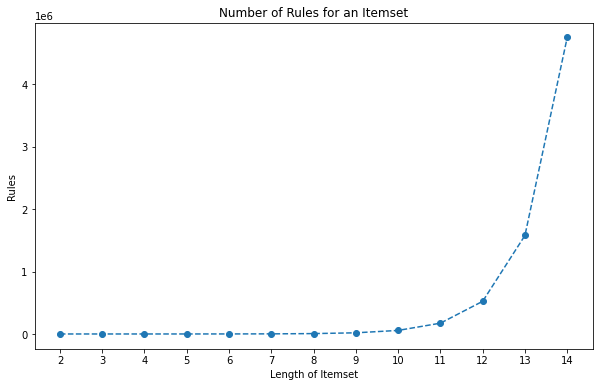
\includegraphics[scale=0.6]{numrules}
\caption{Number of Association Rules for an Itemset}
\label{fig:numrules}
\end{figure}
Given this exponential growth in rules, we can conclude that iterating through all the itemsets, and so a valid solution might be apply the Apriori Algorithm to prune the itemsets. To understand how the algorithm works, the following three metrics must be considered:
The support of a set of products is the fraction of transactions in which these set of products are present. For example,  for a list of transactions $T$, for the product $X$ where $T(X)$ denotes that the set of transactions in which X was present:
\[
\textit{support}(\{A\}) = \frac{T(A)}{T}
\]
and similarly, 
\[
\textit{support}(\abrule) = \frac{T(A,B)}{T}
\]
denotes the support for the rule $\abrule$. Rules with a low support score can be pruned as they indicate a rule does not occur enough to draw any reasonable conclusions from.
\\\textbf{Confidence}\\
Confidence is the measure of how likely a product will be in a basket given that another product is in it. That is to say,  the confidence of a rule $\abrule$ is the conditional probability that $\setB$ occurs in the basket given that $\setA$ is present. The confidence of a rule can be denoted as:
\[
\textit{confidence}(\abrule) = \frac{T(A, B)}{T(A)} \equiv \frac{\textit{support}(\abrule)}{\textit{support}(\setA)}
\]
\\\textbf{Lift}\\
The lift of a rule $\abrule$ is the rise (i.e. \textbf{lift}) that $\setA$ gives to the $\textit{confidence}(\abrule)$.
\[
\textit{lift}(\abrule) = \frac{confidence(\abrule)}{support(\setB)}
\]
For example, consider that $\textit{confidence}(\abrule)=0.5$, and $\textit{support}(\setB)=0.4.$ This means that the presence of $\setA$ increases the probability of $\setB$ being in the same basket by $25\%$ ($\frac{0.5}{0.4}=1.25$), therefore providing us with a lift value of 1.25.  A lift value below 1 would indicate that the occurrence of $\setA$ in a basket decreases the likelihood of $\setB$ occurring in the same basket (i.e. a low product association).
\\
The Apriori principle states that \textit{all subsets of a frequent itemset must be frequent}.  The Apriori principle is a result of the \textit{anti-monotone property of support} \cite{anti_monotone}, which means for $\{A,B,C\}$, $\textit{support}(\{A,B\}) \geq \textit{support}(\{A,B,C\})$.  Therefore, the Apriori principle can be employed to prune the frequent itemsets much more efficiently, because if $support(\{A,B\}) < \textit{min}_{\textit{support}}$, then any itemset containing the set $\{A,B\}$ will also fall below $\textit{min}_{\textit{support}}$. Once the frequent itemsets have been pruned,  association rules can be generated from the remaining itemsets.  The resulting association rules can be even further pruned by removing those that fall below a confidence threshold $\textit{min}_{\textit{confidence}}$.  Finally, the remaining rules can be ranked according to their  lift to find the rules with the highest associations.  Figure \ref{fig:prune} is an illustration of how pruning one set $\{A, B\}$ leads to the pruning of all its children.

\begin{figure}[H]\centering
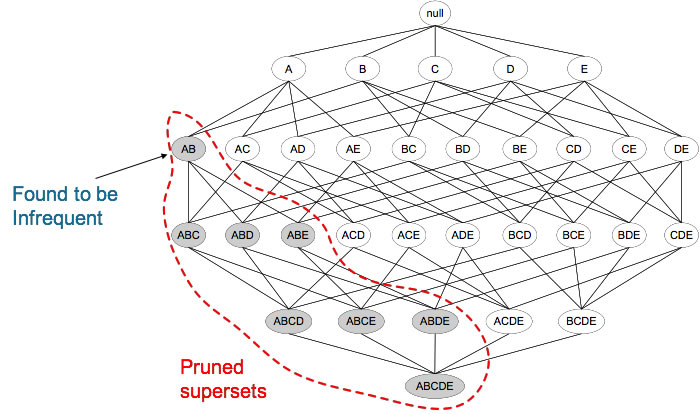
\includegraphics[scale=0.5]{apriori-prune}	
\caption{Pruning Infrequent Rules \cite{apriori-prune}}
\label{fig:prune}
\end{figure}


\section{Related Work}

\subsection{Extracting Minimum Spanning Trees using K-Means}
\textbf{C. Zhong et al.} \cite{kmeans_mst} proposed a novel framework to extract the minimum spanning tree of a graph based on the K-Means clustering algorithm. Their methodology can be separated into two distinct phases. In the first phase,  the data is partitioned into $\sqrt{n}$ clusters via K-Means and the Kruskal's algorithm is applied to each of the clusters individually.  Once the $\sqrt{n}$ MSTs have been constructed, they are combined to form an approximate MST. In the second phase,  new partitions are constructed based on the borders of the clusters identified in phase 1.  Based on these new partitions, a second approximate MST is constructed.  Finally, both graphs are merged such that the resulting graph has $2(n-1)$ edges. The Kruskal's algorithm is run on this graph to get the final approximation of the MST.
\\\textbf{Critical Analysis}\\
The authors have proposed an efficient way to approximate an MST, with their methodology having a complexity of $O(N^{1.5})$, which is faster than the standard MST algorithm which has a complexity of $O(N^2)$. 
For clarity, we have illustrated the disparity between the author's algorithm and the standard algorithm on Figure \ref{fig:speed-compare}.
\begin{figure}[H]
\centering
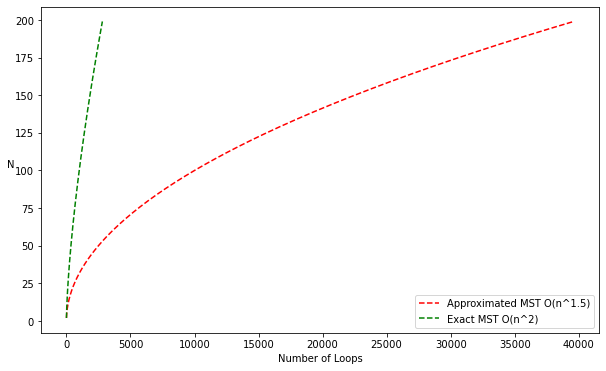
\includegraphics[scale=0.6]{speed-compare} 
\caption{Efficiency of K-Means optimized MST vs.  exact MST}\label{fig:speed-compare}
\end{figure}
\noindent  The K-Means optimized algorithm is $\frac{\sqrt{n}-1}{\sqrt{n}}\%$  faster than the standard MST algorithm.


\subsection{Markov Clustering}
\textbf{S. Dongen} \cite{markov_clustering} introduced the novel Markov Clustering Algorithm (MCL), a graph clustering algorithm that favours sparse graphs (i.e. graphs where the average degree is smaller than the number of nodes). 
The reason for this follows the notion that dense regions in sparse graphs correspond with regions in which the number of $k$-length paths is relatively large - and therefore - paths whose beginnings and ends are in the same dense region have a higher probability for random walks\footnote{A random walk is a stochastic process of of successively random steps along a space, in this case: a directed graph.} of length $k$ as opposed to other paths.
In other words, random walks originating from a node in a dense region have a high probability of ending in that same dense region.
Given a non-negative weighted directional graph $G$, the MCL simulates flow in the graph. 
It does this by first mapping the graph $G$ in a generic way onto a Markov matrix $M_1$.
Once completed, the set of transition probabilities (TP's) are iteratively recomputed via expansion and contraction, resulting in an array of Markov Graphs.
In the expansion stage, higher TP's are calculated, whereas for the contraction phase, a new Markov Graph is created by rewarding high TP's and penalizing low TP's.
The belief is that by doing so, the flow between dense regions that are sparsely connected will be removed, leaving only distinct and unconnected dense regions (i.e. clusters).


\subsection{Apriori Algorithm}
\textbf{R. Aggarwal et al.} \cite{mine} proposed a novel algorithm to generate all statistically significant association rules between items in a database, laying the foundations for association rule mining.  Given a set of items $I = I_1, I_2, I_3,...I_m$, the authors define an association rule to be of the form $X \rightarrow I_j$ where X is a set of items such that $X \in I, I_j \notin X$.  The hypothetical database stated was a list of transactions, $T$, where each transaction $t$ was a binary vector of length $m$, representing a basket purchase, where $t[k] = 1$ if $I_k$ been purchased in that basket.  The authors stated that their methodology for association rule mining could be split into two steps: the generation of candidate itemsets, and the generation of statistically significant association rules from these itemsets. \\
To address the first subproblem, the authors provided the pseudo-code for their candidate itemset generation,  where all itemsets possible were generated from tuples (samples) from the database,  and those itemsets whose support score\footnote{see: Section \ref{mba_define}} is above the minimum support threshold are considered candidates (called \textit{large itemsets}).  Since a brute-force check would be sub-optimal  (the authors note this could take up to $2^m$ passes of the database),  the authors devised a methodology to check for candidate itemsets where on the $k^{th}$ pass of the database, they would only check itemsets of length $k$, to see if they satisfied the support constraint. On the $(k+1)^{th}$ pass, they need only check those itemsets that are 1-extensions (i.e.  itemsets extended by exactly one item) of the \textit{large itemsets} found in the previous pass. This is because of what would later be known as the \textit{Apriori Principle}, where if an itemset $Y$ is \textit{large}, then all subsets of $Y$ must also be \textit{large}. Therefore, if they found the itemset $\{A,B\}$ was \textit{small} (i.e. did not satisfy the support constraint), then sets containing $\{A,B\}$ (e.g. $\{A,B, C\}, \{A,B, D\}, \{A,B, C, D\}$) would also be small, and need not be checked. This means, however, that if an itemset $I$ is \textit{large}, then another pass over the dataset would be required to check the support of the subsets of $I$. To avoid this, the authors devised a measure to calculate the expected support, $\bar{s}$, of an itemset,  and use this to measure the support of itemsets $I = (X + I_j)$ not only where $I$ is expected to be large, but also where $X+I_j$ is expected to be small but $X$ is expected to be large, further helping them prune the number of itemsets to check.  The authors proceed to define a method that allows the algorithm to be more memory efficient\footnote{This may no longer be required due to the advances in computational power in the the 27 years since this paper was written.}. The authors also defined method to further prune itemsets from the search, namely \textit{remaining tuples optimization} and \textit{pruning function optimization}.\\
To address the second subprobem,  the authors proposed the following methodology: for each large itemset $Y = I_1, I_2,...I_k, k\geq 2$ from the set of non-pruned large itemsets, generate a set of association rules of form $X \rightarrow I_j$ such that the consequent is $I_j$ and the antecedent (i.e. the precedent set in the rule) is a subset $X$ of $Y$ such that $X$ is of length $k-1$ and $I_j \notin X$. Therefore, each large itemset will produce $k$ rules. From the generated rules, the authors discarded those rules whose confidence scores\footnote{see: Section \ref{mba_define}} fell below the minimum confidence threshold $c$.\\
The authors tested their methodology on a sales dataset with $46,783$ transactions,  with $63$ \textit{items} (in this case, the department from which the customer bought an item). They used a configuration of a minimum support threshold of $1\%$ and a minimum confidence threshold of $50\%$. The rules produced seemed to follow with general intuition, such as:\\
$\{\text{Auto Accessories, Tires}\} \rightarrow \{\text{Automotive Services}\} $\\
Furthermore, the authors assessed the accuracy of their expectation method, by measuring the ratio of correctly estimated itemsets for both small and large, against various values for the minimum support threshold, and visualizing the result. To isolate the effect of their expectation method, they disabled their pruning optimization functions. They were able to conclude that their estimation accuracy was satisfactory, as their accuracy was above 98\% for support thresholds except the first, where it was 96\%.  The authors also tested the effectiveness of their pruning optimization functions, namely the \textit{remaining tuples} and the \textit{pruning function} optimization functions, against multiple minimum support threshold values. They were able to conclude that their pruning efficiency increased as the support threshold increased.
\\\textbf{Critical Analysis}\\
The authors have proposed a novel methodology that has been the bedrock of numerous research publications,  including most of the papers in this literature review.  Their estimation function performed with high accuracy, meaning it can reduce the number of passes through a database the algorithm has to take by a significant amount. Additionally, their pruning techniques allowed them to eliminate a large proportion of itemsets from the space. Even after the significant pruning of rules, a major drawback of this methodology is the large number of rules produced, although one could argue that only the highest performing rules need be observed in further detail.


\subsection{Subjective Measurement of Association Rules}
\textbf{M. Zekić-Sušac et al.} \cite{market_ass} proposed a novel measure for the \textit{interestingness} of association rules,  identifying that a dominant, universally used measure did not exist. The authors' goal was to combine objective measures such as the support, confidence and lift scores with more subjective measures. Instead of the Apriori approach, their methodology has them generate association rules via the \textit{tree-building technique} - which compresses a large database into a Frequent-Pattern tree, citing that this technique was more efficient than the Apriori algorithm. The author's employed the heuristical unexpectedness measure(i.e.  significantly contradicting a user's prior beliefs) and the heuristical actionability measure (i.e. if the end user can use the information to their advantage(e.g. a promotion)) as their subjective measures, and a minimum confidence threshold of 51\% as their subjective measure.  Since a subjective measure would require a human subject, the authors' used the estimations of a sales manager from a Croatian retail chain, and stored his responses in binary format for the subjective measures (i.e. 0 if a rule was unexpected else 1, 0 if a rule is not useful else 1). The dataset used for this paper was a real transactional dataset with 14,012 transactions and a set of 1,230 unique items (which was later pruned to 7,006 transactions and a set of 278 products) from the same Croatian retail chain their test subject worked at. The authors then generated association rules from the first-level hierarchical grouping of items from the dataset (items with a minimum support of 25\%),  of which 36 rules were identified as statistically significant.  From this set of rules, only two rules satisfied both subjective measures and the confidence constraint, and therefore these two rules were identified as highly interesting.  The authors then generated association rules from the second-level hierarchical grouping of items, where items that represented the same product (but had different a manufacturer, brand etc.) were grouped together. Of the rules generated, 15 satisfied their confidence constraints and had a support value able 10\%. 5 rules from this set satisfied both their subjective and objective measures,  more than the previous experiment  The authors were able to conclude that the increase in accuracy and number of interesting rules resulted from the second level of grouping which generalized the products.\\
\textbf{Critical Analysis}\\
Wheras the original measure of statistical significance introduced by R. Aggarwal et al.  was purely objective, the authors  of this paper have presented a well thought out approach to combining the subjective metrics with objective ones to produce a human-verified association rule set.  A few caveats to note, however: their study only involved one subject, which is rarely regarded to be statistically acceptable. An ideal study would require multiple, randomly chosen subjects to offset any bias that the singular subject would have had, and in addition, the larger their subject size, the closer their collective estimations will model the total population's.  Another drawback of their approach is that by using human intuition as a metric,  they're promoting association rules that satisfy pre-existing notions about human behavior (e.g. if someone buys milk, they'll \textit{probably} get eggs too), however these types of rules are usually regarded as common knowledge,  whereas the beauty of association rule mining is in its ability to surface association rules that - while true - seem unintuitive, and therefore are less likely to be known by the management of such organizations.


% MAIN MST PAPER
\subsection{Association Rules from Minimum Spanning Trees}
\label{sec:mst paper}
\textbf{M. A. Valle et al.} \cite{mst_paper} proposed a novel methodology to study the structure and behavior of consumer market baskets from the topology of a minimum spanning tree which represented the interdependencies between products, and use this information to complement the association rule generation process. The input to their proposed methodology was a correlation matrix between the set of all one-hot encoded purchase vectors such that each vector denoted the presence or non-presence of each product from the dataset in that vector.  The dataset used for the MST construction was a list of $1,046,804$ transactions containing a set of $3,240$ unique products from a large supermarket chain branch in Santiago, Chile.  When building this correlation matrix, the authors opted to use the Pearson's Coefficient (which is equivalent to the coefficient $\phi$ for binary data such as theirs) over the traditionally used Jaccard distance to compute the similarity between the binary product vectors, as the former provides both a positive and negative association between products. Additionally,  they used the distance function $d_{ij} = \sqrt{2(1-\phi_{ij}}$ to transform the correlation matrix into a distance measurement (i.e. the weight of the edges).  The authors constructed a MST for 220 product subcategories, and noted that there was a significant level of grouping between product sub-categories that belonged to the same parent category.  To remove edges from the MST that were not statistically significant,  the authors used the mutual information \cite{measure} measure $\sum\limits_{x,y}log_2 \frac{r(x,y)}{p(x)q(y)}$ between product subcategories $p$ and $q$, and were able to prune 14 edges, all of which were connected to a terminal node, therefore effectively pruning 14 vertices from the MST too. To identify the most influential regions of the MST, the authors defined an influence zone of distances that were in the $10^{th}$ percentile. To generate meaningful association rules,  for each MST product $i$, the authors ran a search for the set of all association rules $R_i$ such that $P_i \rightarrow P_j (i \neq q)$. Then from the resulting set of rules, they searched for rules that obeyed $P_i \rightarrow P_m$ where $m$ a product node connected to the product $i$ in the minimum spanning tree.  For both resulting sets of rules for each product, the mean of their lift scores were observed, and the authors determined that the rules that were reinforced by the MST had a higher mean, and that a majority of these rules had a lift score above the $90^{th}$ percentile. 
\\
To identify the clusters each of the products should be identified under, the authors constructed a hierarchical tree using the average linkage clustering method, and by using an unspecified cut distance, they were able to produce 17 taxonomic groups (i.e. clusters). Cross-referencing their results with the actual parent categories of the products, they were able to conclude that the MST did indeed categorize the product sub-categories into clusters with a reasonable degree of accuracy. The authors then compared their MST to another methodology, namely the structured association map (SAM) \cite{kim}, using the Jaccard distance as a measure of similarity,  and were able to generate interesting 2x2 rules (i.e. $\{A,B\}\rightarrow\{C, D\}$), all with lift scores above 1.0, with one rule even having a lift score of 106.46. They concluded that while both approaches provided different information, they both visually identify the strongest relationships between the products, and provide useful information to reduce the search space for association rules.
\\\textbf{Critical Analysis}\\
The authors' approach seems to be novel,  thorough and well structured.  Their methodology successfully employed the use of minimum spanning trees to complement the association rule generation process with sound results.  One caveat of their approach is that they only used the MST to generate single-element rules (i.e. $\abrule$, where the antecedent and consequent contain only one element each). Using the distance score in conjunction with the importance function they defined (i.e. $\sum\limits_{k \in K_u}^{} \frac{1}{w_{uk}}$), they could have defined a system to produce multi-element rules (i.e. where either/both the antecedent and the consequent have more than one element), then rank them using their respective lifts. While single-element rules are easily understandable and tend to have high lift values when extracted from the MST, multi-element rules would provide an additional layer of insight as to how a range of products (perhaps a cluster) related to another.


\subsection{Summary}
In conclusion, \textbf{R. Aggarwal et al.} introduced a formal system for association rules, and a method to generate them from a transactional database - the Apriori Algorithm \cite{apriori}.  However, while these papers only based the interestingness of an association rule on objective measures such as the support, confidence and lift scores of these rules, \textbf{M. Zekić-Sušac et al.} proposed a methodology where subjective human input was used to validate the interestingness of these rules. A drawback of the above methods, however, is the large number of rules produced. \textbf{M. A. Valle et al.} introduced a methodology to extract high value association rules from a minimum spanning tree, used to complement the rules produced by the Apriori algorithm. A caveat of this approach, however, is that it can only produce rules such that the antecedent and consequent are sets with one element each. Additionally, the methodology described involves building the MST using Prim's algorithm, which can be relatively slow. \textbf{C. Zhong et al.} proposed a solution to this, where the Kruskal's algorithm was optimized using K-Means, leading to a significant performance increase as illustrated in Figure \ref{fig:speed-compare}. The methodology proposed in this paper was a framework of sorts, where Kruskal's could be substituted with any MST algorithm, such as Prim's.
All the research conducted above has served as the inspiration for this project.


\chapter{Multi-Element Association Rule Generation}
\section{[Creation/Organization/Blank]}

\section{MST Generation}

\section{Testing and Evaluation}
\section{Metrics}
\section{Data Filtering}
Talk about how MST different when comparing different cities.

% References
\printbibliography[heading=bibintoc, title=References]

% ------------------------------------------------------------------------------
% End document
% ------------------------------------------------------------------------------
\end{document}
